
\documentclass[14pt]{matmex-diploma-custom}
\usepackage{graphicx}
\usepackage{float}
\graphicspath{ {./images/} }

\begin{document}
\filltitle{ru}{
    chair              = {Математическое обеспечение и администрирование информационных систем},
    title              = {Разработка сервиса для подсчета объема круглого леса: система подписок, интерфейс выделения области интереса},
    type               = {diploma},
    position           = {студента},
    group              = 244,
    author             = {Паршин Максим Алексеевич},
    supervisorPosition = {к.\,т.\,н., доцент},
    supervisor         = {Литвинов Ю.\,В.},
    reviewerPosition   = {директор продуктовых разработок\\ ООО <<Системы Компьютерного Зрения>>\\},
    reviewer           = {Елисеева Т.\,В.},
}
\maketitle
\tableofcontents

\section*{Введение}

Одним из необходимых этапов производства целлюлозно-бумажной и прочей продукции, изготавливаемой из древесного сырья, является приёмка поставляемого на комбинаты круглого леса. Данный процесс включает в себя измерение и оценку таких параметров штабеля, как длина, ширина, объем, коэффициент полнодревесности. На большинстве предприятий приёмка проводится инженерами при помощи ручных замеров линейкой, что требует много времени и сил. При этом всегда существует вероятность человеческой ошибки, и точность таких замеров может быть подвергнута сомнению.

Цель проекта, работу над которым ведет компания <<Системы Компьютерного Зрения>>, --- автоматизировать и упростить процесс приемки сырья на лесоообрабатывающих предприятиях, разработав сервис, использующий методы машинного обучения для детекции торцов бревен на изображении и рассчитывающий необходимые параметры по полученным данным.


\section*{Постановка задачи}

Для достижения цели перед автором были поставлены следующие задачи:

\begin{itemize}  
\item реализовать систему подписок для ограничения доступа пользователей к функциональности в зависимости от тарифного плана;
\item реализовать интерфейс выделения области интереса на изображении в мобильном приложении;
\item реализовать локализацию мобильного приложения для англоговорящих пользователей;
\item автоматизировать процесс сборки мобильного приложения.
\end{itemize}

\section*{Обзор проекта}

Работа сервиса <<SmartTimber>> \cite{timberweb} основана на взаимодействии следующих модулей:

\begin{itemize}  
\item мобильного приложения для операционной системы Android, выступающего в качестве тонкого клиента и предоставляющего пользовательский интерфейс;
\item серверного приложения, получающего данные от клиента и осуществляющего детекцию торцов бревен и расчёт параметров.
\end{itemize}

 Основной сценарий использования сервиса пользователем включает в себя следующие действия:
 
\begin{itemize}  
\item загрузка изображения штабеля из галереи или создание нового снимка;
\item отметка предмета-эталона длины на изображении;
\item выделение на изображении многоугольной области, внутри которой будет происходить детекция;
\item ввод параметров расчёта: длины отмеченного эталона, породы древесины, типа сортимента;
\item отправка данных на сервер;
\item детекция торцов бревен при помощи нейросети и расчёт объема, ширины и высоты штабеля, коэффициента полнодревесности;
\item получение результатов с сервера;
\item просмотр результатов с последующим опциональным сохранением.
\end{itemize}

Весной 2020 года началось пилотное тестирование сервиса в сотрудничестве <<Систем Компьютерного Зрения>> с некоторыми крупными российскими лесообрабатывающими предприятиями \cite{vedomosti}.

Разработка серверной части ведется на платформе ASP.NET MVC, мобильной части --- на платформе Xamarin.Forms.

 \section*{Обзор использованных инструментов}
 
 \subsection*{SkiaSharp}

SkiaSharp --- графическая библиотека для платформы .NET Framework, применяемая для отрисовки различных геометрических форм и изображений. Данная библиотека была использована как автором при работе над интерфейсом выделения области интереса на изображении, так и другими разработчиками для реализации интерфейса отметки предмета-эталона. Среди преимуществ SkiaSharp следует отметить её происхождение от библиотеки Skia, разрабатываемой Google, и подробную документацию, содержащую готовые реализации некоторых часто встречаемых задач \cite{skia}.

\subsection*{Entity Framework}

Для хранения информации о пользователях серверной частью уже использовалась платформа Entity Framework, разрабатываемая Microsoft и являющаяся распространённой ORM-системой, применяемой при разработке веб-приложений на ASP.NET, поэтому она была выбрана и в целях организации данных о подписках. 

\subsection*{Owin-Authorization}

Для реализации авторизации пользователей с различными подписками использовался механизм Claims (утверждений), предоставляемый ASP.NET и предназначенный для хранения некоторой информации о статусе пользователя, в данном случае, о факте наличия у него действующей подписки и её типа. Однако ASP.NET MVC, в отличие от более современной и распространённой на данный момент платформы ASP.NET Core, не имеет удобного API для ограничения действий пользователя в зависимости от утверждений о нем. В связи с этим возникла необходимость использования библиотеки, портирующей данную функциональность с ASP.NET Core на ASP.NET MVC, и разработанной пользователем GitHub DavidParks8 \cite{auth}.

\subsection*{Jenkins}

Так как одной из задач, поставленных перед автором, стала автоматизация сборки мобильного приложения, возникла проблема выбора подходящей для этих целей системы непрерывной интеграции. В результате предпочтение было отдано серверу Jenkins с открытым исходным кодом, поскольку компанией был предоставлен серверный компьютер для нужд проекта, а большинство других решений, таких как Microsoft Azure Pipelines, предоставляет собственные вычислительные мощности, в связи с чем распространяется на платной основе. Другое преимущество Jenkins --- наличие большого количества плагинов, созданных сообществом, к примеру, использованный в проекте плагин для рассылки уведомлений о сборке в Slack.

\section*{Реализация}


\subsection*{Система подписок}

Для хранения данных о подписках на сервере была реализована архитектура базы данных, включающая в себя следующие классы-сущности (Рис. \ref{database}): 

\begin{itemize}  
\item сущность \textbf{Subscription}, представляющая тарифный план и связанная отношением <<многие-ко-многим>> при помощи класса\\ UserSubscription с уже существующей сущностью User, используемой для представления пользователя. Тарифный план имеет свойства, задающие его название, цену, стандартный период и состояние (архивный или нет);
\item сущность \textbf{UserSubscription} реализовывает связь <<многие-ко-многим>> между классами User и Subscription, используется для представления факта приобретения подписки конкретным пользователем и имеет соответствующие свойства: идентификаторы пользователя и тарифного плана, дату покупки и дату окончания.
\end{itemize}

\begin{figure}[h]
\centering
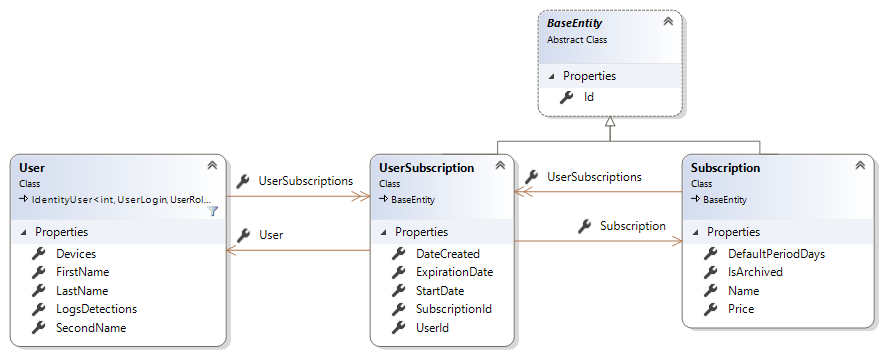
\includegraphics[width=\textwidth]{database.png}
\caption{Архитектура базы данных}
\label{database}
\end{figure}

Проверка наличия действующей подписки у пользователя происходит следующим образом (Рис. \ref{subscriptions}): пользователь с помощью мобильного приложения отправляет HTTP-запрос к некоторому методу сервера. Сервер, используя существующий механизм авторизации, получает доступ к объекту, представляющему данного пользователя, и обращается к реализованному классу ClaimsTransformerComponent. Его задача --- проверить по базе наличие какой-либо подписки у пользователя, и выдать ему на основании полученных данных утверждение (Claim) со значением, соответствующим тарифному плану, если имеется действующая подписка. Далее происходит обращение к запрашиваемому методу, и, так как он помечен атрибутом Authorize, реализованным в библиотеке Owin-Authorization, управление передается объекту класса SubscriptionRequirementHandler, который проверяет имеющийся у пользователя список выданных ему утверждений и передает управление целевому методу, если найдено необходимое утверждение, в противном случае возвращает результат, свидетельствующий об ошибке авторизации.

\begin{figure}[h]
\centering
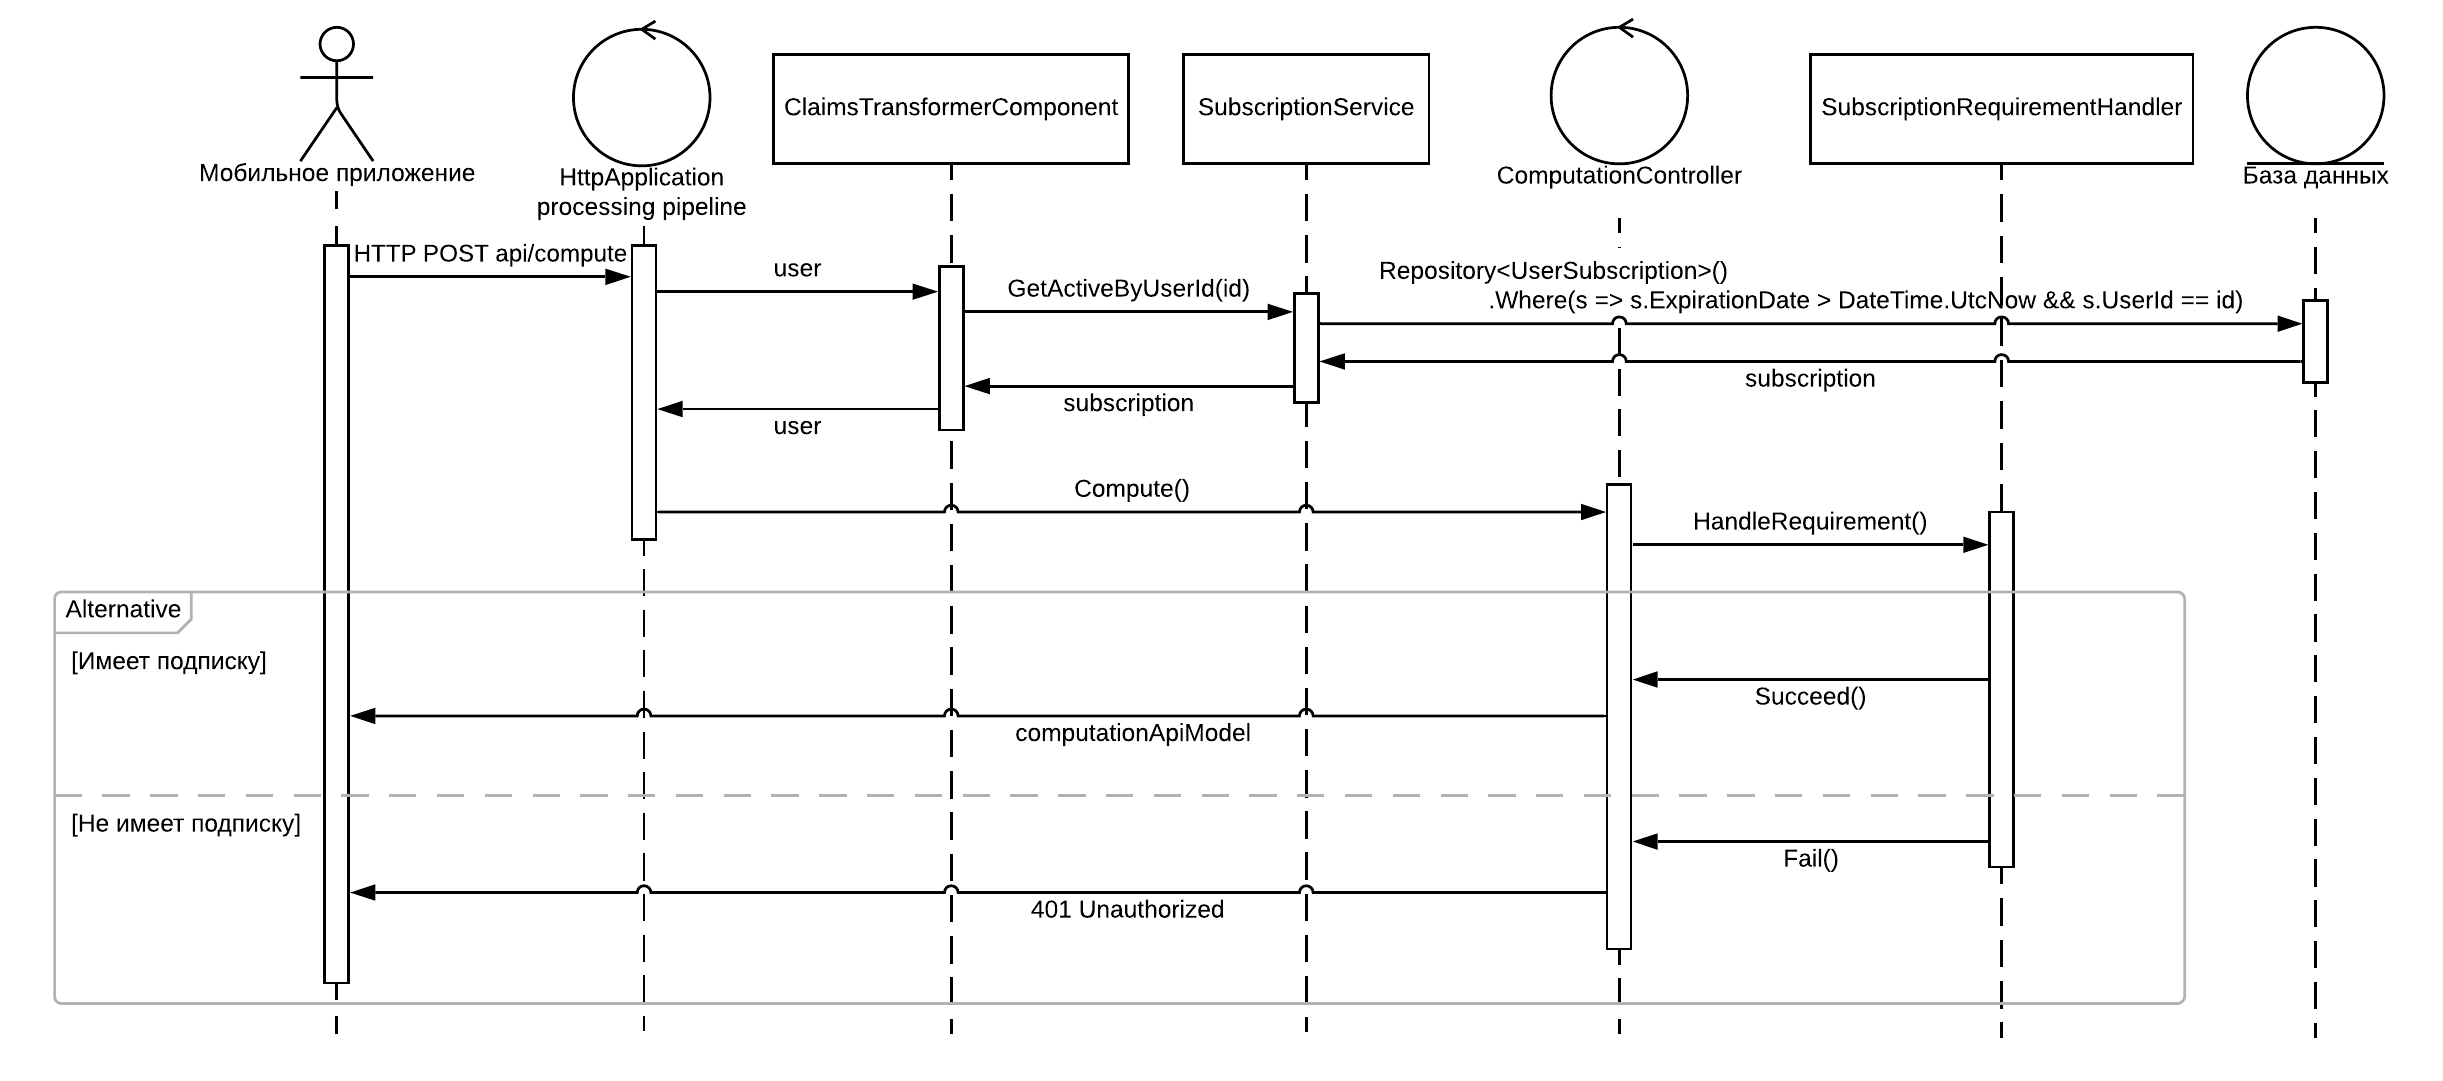
\includegraphics[width=\textwidth]{subscriptions.png}
\caption{Диаграмма последовательности проверки наличия подписки}
\label{subscriptions}
\end{figure}

\subsection*{Интерфейс выделения области интереса}

Для выделения области интереса на изображении пользователю предоставляется возможность ограничить ее многоугольником (Рис. \ref{areascreen}). При переходе на экран область представляет собой прямоугольник, далее имеется возможность жестами двигать вершины и добавлять новые.

Основной проблемой, возникшей в процессе работы над задачей, стала необходимость проверки получающегося многоугольника на самопересечения. В результате был применен следующий алгоритм: происходит определение вершины, которая была сдвинута, и две стороны многоугольника, соединённые ей, проверяются на пересечение со всеми остальными сторонами. Для этого рассматривается несколько троек вершин для каждой пары отрезков \cite{intersection}, проверяемых на пересечение, и рассчитывается их ориентация на плоскости (точки тройки могут лежать на одной прямой либо идти по часовой стрелке или против часовой стрелки). Затем ориентации троек сравниваются между собой, и в зависимости от количества совпадений ориентаций делается вывод о наличии пересечения у отрезков. В результате, если выясняется, что сдвиг точки пользователем приводит к самопересечению многоугольника, данное действие блокируется.

\begin{figure}[h]
\centering
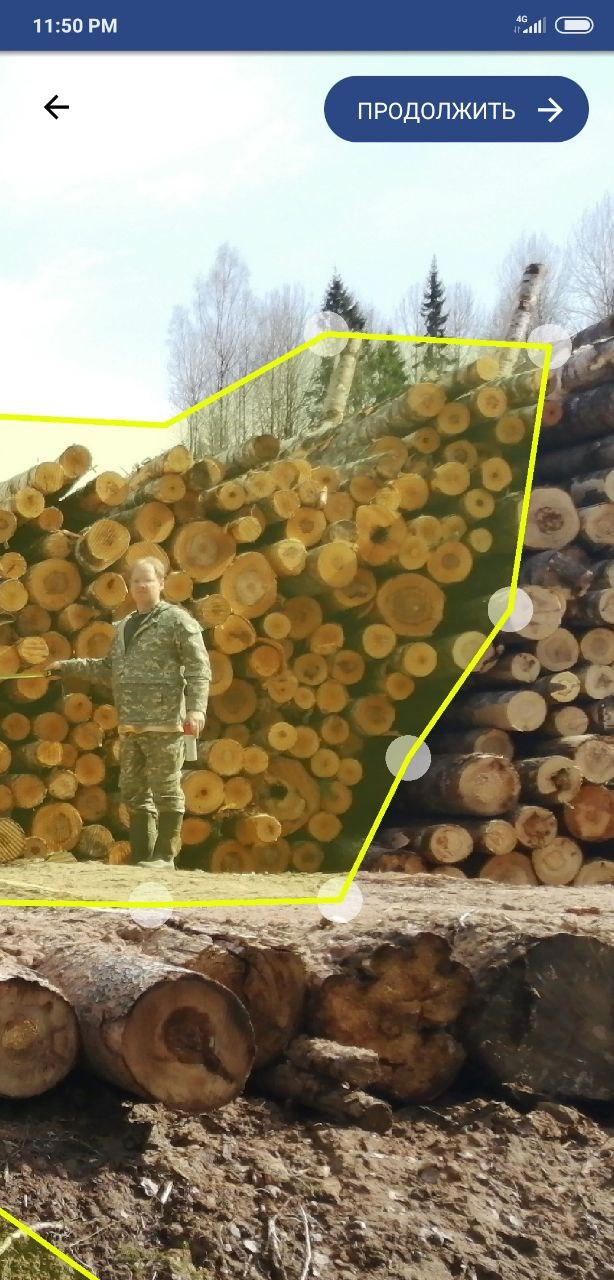
\includegraphics[scale=0.30]{areascreen.png}
\caption{Графический интерфейс экрана выделения области интереса}
\label{areascreen}
\end{figure}

\subsection*{Локализация}

Что касается локализации, она была реализована стандартным для Xamarin-приложений образом. В проект добавлены два файла строковых ресурсов (ключ-значение), соответствующих русскоязычной и англоязычной версиям. В исходном коде приложения при необходимости обращения к строке, которая должна быть локализована, используется ключ её ресурса. Файл, из которого читается значение, автоматически выбирается в зависимости от языка устройства.

\subsection*{Непрерывная интеграция}

Сервис непрерывной интеграции развернут на собственном сервере компании. Сборка проекта происходит автоматически при изменениях в Bitbucket-репозитории. Если сборка завершилась успешно, установочный файл Android-приложения отправляется в Slack-канал, используемый командой.

\newpage
\section*{Результаты}

\begin{itemize}  
\item Реализована система подписок и механизм ограничения доступа пользователей с различными тарифными планами.
\item Реализован интерфейс выделения области интереса в мобильном приложении.
\item Реализована локализация для англоговорящих пользователей.
\item Сборка мобильного приложения автоматизирована.
\item Результаты внедрены в серверную и мобильную части.
\end{itemize}

\setmonofont[Mapping=tex-text]{CMU Typewriter Text}
\bibliographystyle{ugost2008ls}
\bibliography{report.bib}
\end{document}
